
% \begin{frame}{Usage}

%     Linear RNNs opens up the modeling design space

%     \vspace{1cm}
%     \begin{itemize}
%         \item How to efficiently calculate?
%         \item How to parameterize?
%     \end{itemize}
% \end{frame}

% \begin{frame}{Calculation}
%     Recall the main calculation is a $L$ length convolution, 
    
%     \begin{figure}
%         \centering
%         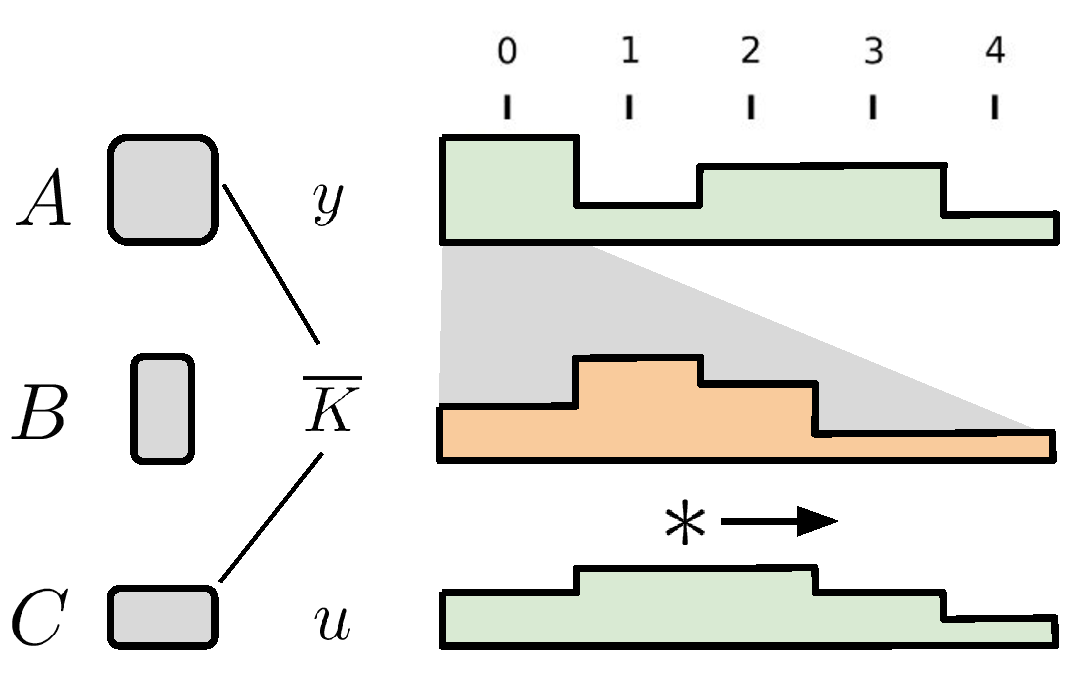
\includegraphics[width=0.7\textwidth]{Figs/SSM.pdf}
%         \label{fig:my_label}
%     \end{figure}
% \end{frame}



\begin{frame}{Method 2: Parallel Associative Scan \cite{smith2022simplified} }
    Compute $e_1\bullet \ldots \bullet e_l$ for any associative operator $\bullet$

\begin{center}
\Tree [.$\bullet$ [.$\bullet$ [.$\bullet$ $e_1$ ] [.$\bullet$ $e_2$ ] ] [.$\bullet$ [.$\bullet$ $e_3$ ] [.$\bullet$ $e_4$ ] ] ]
    
\end{center}
    \cite{Blelloch1990-yo,Martin2018-bq}
\end{frame}

\begin{frame}{}
    \[e_k = (\boldsymbol{E}_k, \boldsymbol{e}_k) = (\bar{\textcolor{green}{\boldsymbol{A}}}, \bar{\textcolor{blue}{\boldsymbol{B}}}u_k)\]
    \begin{figure}
        \centering
        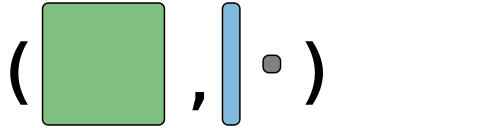
\includegraphics[height=0.1\textwidth,clip,trim={0cm 0cm 5cm 0cm}]{Figs/assoc.png}
        \label{fig:my_label}
    \end{figure}

    \[e_i \bullet e_j = (\boldsymbol{E}_i \boldsymbol{E}_j, \boldsymbol{E}_j \boldsymbol{e}_i + \boldsymbol{e}_j ) \]
    \begin{figure}
        \centering
        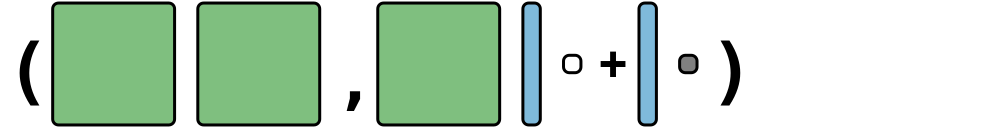
\includegraphics[height=0.1\textwidth,clip,trim={0cm 0cm 6cm 0cm}]{Figs/assoc2.png}
    \end{figure}
\end{frame}



% \begin{frame}{Parmeterization of RNN Models}
%     SSM framing gives an elegant parameterization of Linear RNNs,

%     \begin{figure}
%         \centering
%         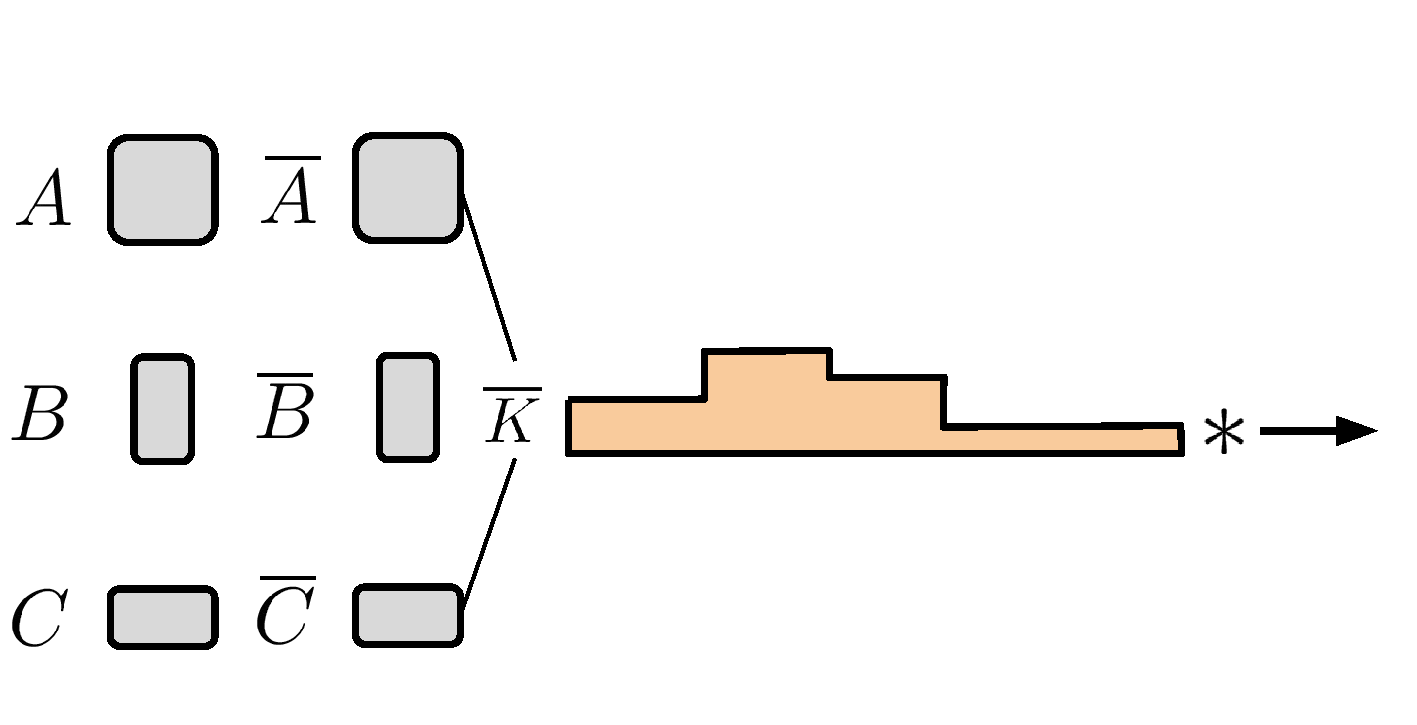
\includegraphics[width=0.7\textwidth]{Figs/SSMParam.pdf}
%         \label{fig:my_label}
%     \end{figure}

%     Researchers have explored other parameterizations
% \end{frame}











